%%%%%%%%%%%%%%%%%%%%%%%%%%%%%%%%%%%%%%%%%
% Beamer Presentation
% LaTeX Template
% Version 1.0 (10/11/12)
%
% This template has been downloaded from:
% http://www.LaTeXTemplates.com
%
% License:
% CC BY-NC-SA 3.0 (http://creativecommons.org/licenses/by-nc-sa/3.0/)
%
%%%%%%%%%%%%%%%%%%%%%%%%%%%%%%%%%%%%%%%%%

%----------------------------------------------------------------------------------------
%	PACKAGES AND THEMES
%----------------------------------------------------------------------------------------

\documentclass{beamer}

\mode<presentation> {
\usetheme{Warsaw}
\usetheme{metropolis}  
%\setbeamertemplate{footline} % To remove the footer line in all slides uncomment this line
%\setbeamertemplate{footline}[page number] % To replace the footer line in all slides with a simple slide count uncomment this line

%\setbeamertemplate{navigation symbols}{} % To remove the navigation symbols from the bottom of all slides uncomment this line
}
%\setbeamertemplate{background}
%{\includegraphics[width=\paperwidth,height=\paperheight,keepaspectratio]{background.jpg}}
\usepackage{graphicx} % Allows including images
\usepackage{booktabs} % Allows the use of \toprule, \midrule and \bottomrule in tables
\definecolor{cerulean}{rgb}{0.0, 0.48, 0.65}
\definecolor{cinnamon}{rgb}{0.82, 0.41, 0.12}
%----------------------------------------------------------------------------------------
%	TITLE PAGE
%----------------------------------------------------------------------------------------

\title[GECO ]{STREAM 3D project} % The short title appears at the bottom of every slide, the full title is only on the title page

\author{D. Cerroni, L. Formaggia, A. Scotti and P. Zunino} % Your name
\institute[MOX laboratory, Department of Mathematics] 
{
Politecnico di Milano\\ % Your institution for the title page
\medskip
%\textit{daniele.cerroni} % Your email address
}
\date{\today} % Date, can be changed to a custom date
\usepackage{tikz}
\usetikzlibrary{mindmap,trees, positioning}
\usepackage{adjustbox}
%%%%%%%%blocks
\usetikzlibrary{shapes,arrows}
\tikzstyle{decision} = [diamond, draw, fill=blue!20, text width=4.5em, text badly centered, node distance=3cm, inner sep=0pt]
\tikzstyle{block} = [rectangle, draw, fill=blue!20, text width=15em, text centered, rounded corners, minimum height=4em]
\tikzstyle{line} = [draw, -latex    ]
\tikzstyle{cloud} = [draw, ellipse,fill=red!20, node distance=3cm, minimum height=2em]

\usepackage{amsmath}
\usepackage{verbatim}
\usetikzlibrary{arrows,shapes}
\renewcommand\mathfamilydefault{\rmdefault}
  % put color to \boxed math command
\newcommand*{\boxcolor}{orange}
\makeatletter
\renewcommand{\boxed}[2]{\textcolor{#2}{%
\tikz[baseline={([yshift=-1ex]current bounding box.center)}] \node [rectangle, minimum width=1ex,rounded corners,fill=#2!40,draw] {\normalcolor\m@th$\displaystyle#1$};}}
 \makeatother


\setbeamertemplate{background}
{
\includegraphics[width=\paperwidth,height=\paperheight]{figure/back}}

\begin{document}

\begin{frame}
\titlepage % Print the title page as the first slide
\end{frame}
%%%%%%%%%%%%%%%%%%%%%%%%%%%%%%%%%%%%%%%%%%%%%
\begin{frame}
\frametitle{Overview} % Table of contents slide, comment this block out to remove it
\tableofcontents % Throughout your presentation, if you choose to use \section{} and \subsection{} commands, these will automatically be printed on this slide as an overview of your presentation
\end{frame}
%%%%%%%%%%%%%%%%%%%%%%%%%%%%%%%%%%%%%%%%%%%%%%%
\section{Introduction}
%%%%%%%%%%%%%%%%%%%%%%%%%%%%%%%%%%%%%%%%%%%%%%%
\begin{frame}{Background and Motivations}
\begin{columns}
\begin{column}{0.65\textwidth}
\begin{block}{Key processes of sedimentary basin evolution:} 
\begin {itemize}
\item  geomechanics and dynamic evolution of stress and deformations; 
\item  transport of dissolved chemicals; 
\item geochemical reactive processes.
\end{itemize}
\end{block}
\end{column}
\begin{column}{0.35\textwidth}
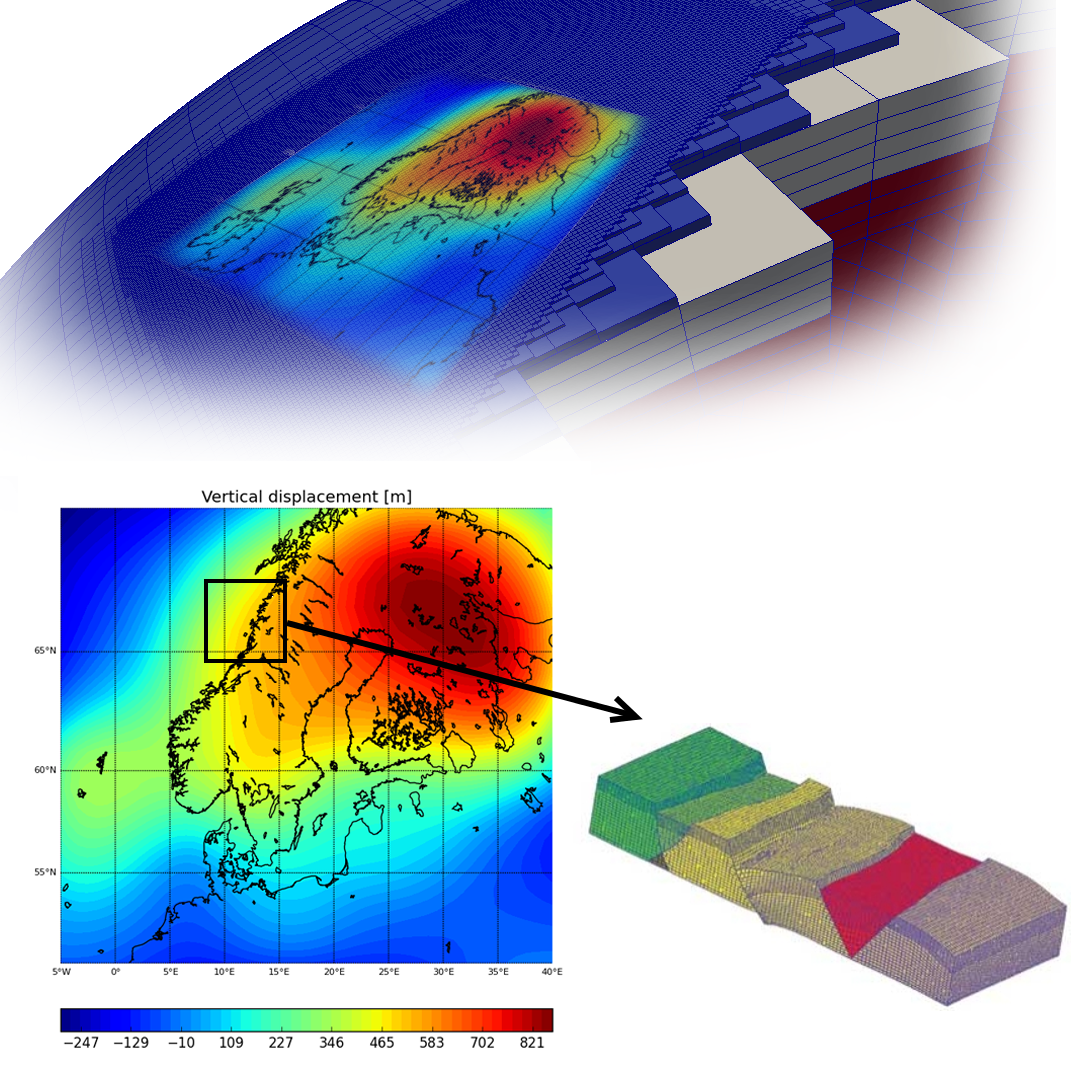
\includegraphics[width=0.9\textwidth]{figure/intro1}
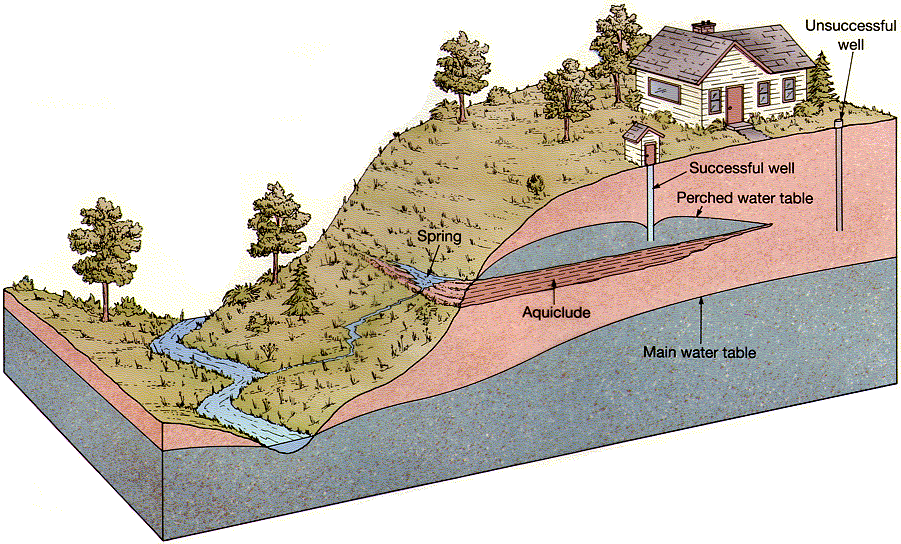
\includegraphics[width=0.9\textwidth]{figure/aquafier}
\end{column}
\end{columns}
\end{frame}
%%%%%%%%%%%%%%%%%%%%%%%%%%%%%%%%%%%%%%%%%%%%%%%
\begin{frame}{Background and Motivations}
\centering
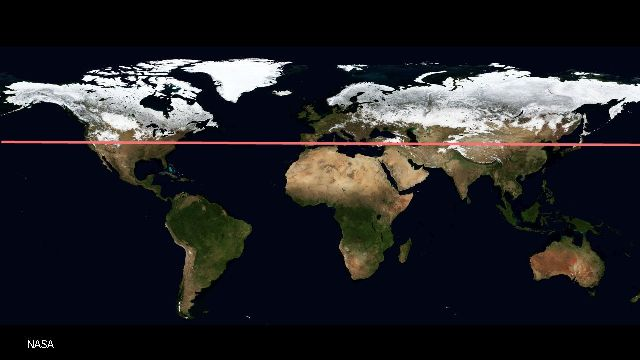
\includegraphics[width=0.9\textwidth]{figure/ice_age_snows}
\end{frame}
%%%%%%%%%%%%%%%%%%%%%%%%%%%%%%%%%%%%%%%%%%%%%%%
\begin{frame}{Background and Motivations}
\begin{columns}
\begin{column}{0.45\textwidth}
\begin{block}{The effects of glaciations on the subsurface:} 
\begin {itemize}
\item  the mechanical compaction due to the load of ice sheets; 
\item  the deformation of the lithosphere by isostasy; 
\item  the subglacial meltwater; 
\item  the generation of permafrost. 
\end{itemize}
\end{block}
\end{column}
\begin{column}{0.5\textwidth}
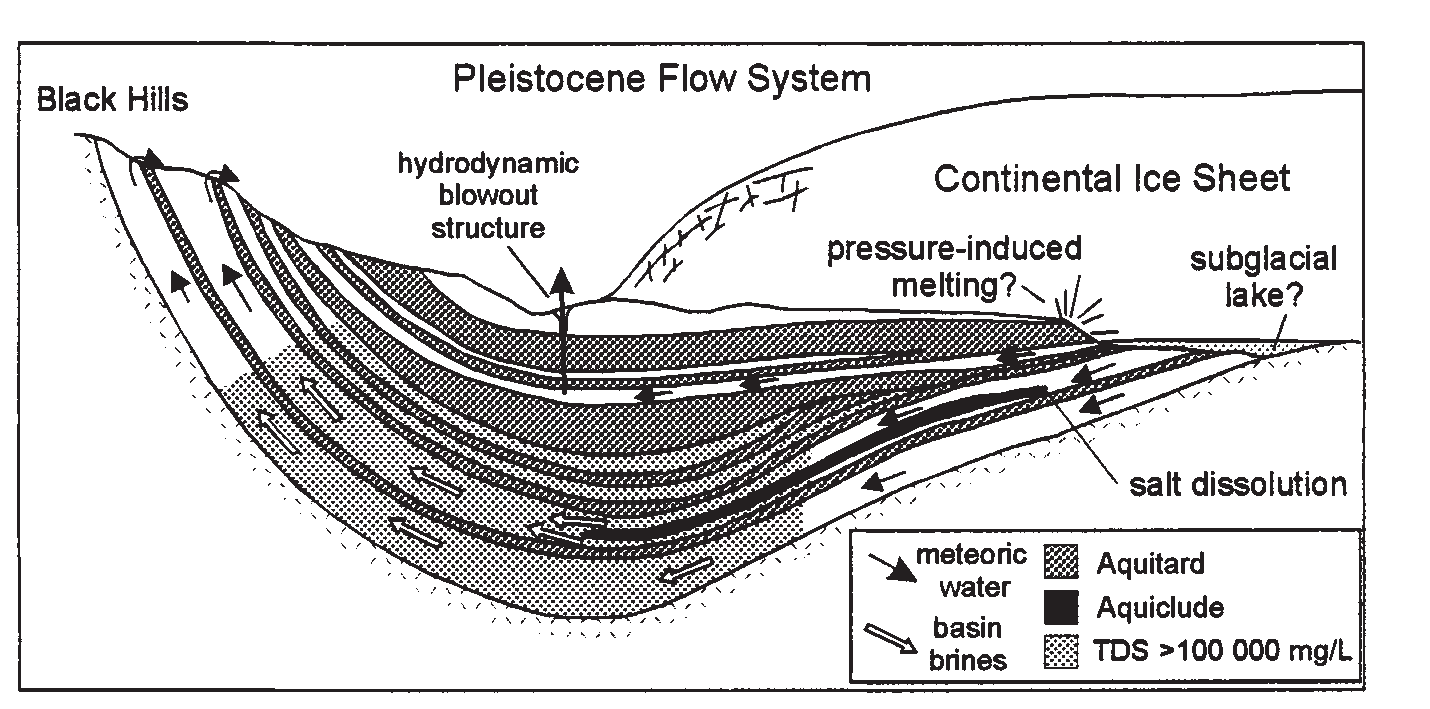
\includegraphics[width=0.9\textwidth]{figure/basin_glacial}
\end{column}
\end{columns}
\end{frame}
%%%%%%%%%%%%%%%%%%%%%%%%%%%%%%%%%%%%%%%%%%%%%%%
\begin{frame}{Conceptual}
\begin{adjustbox}{max totalsize={.9\textwidth}{.7\textheight},center}
 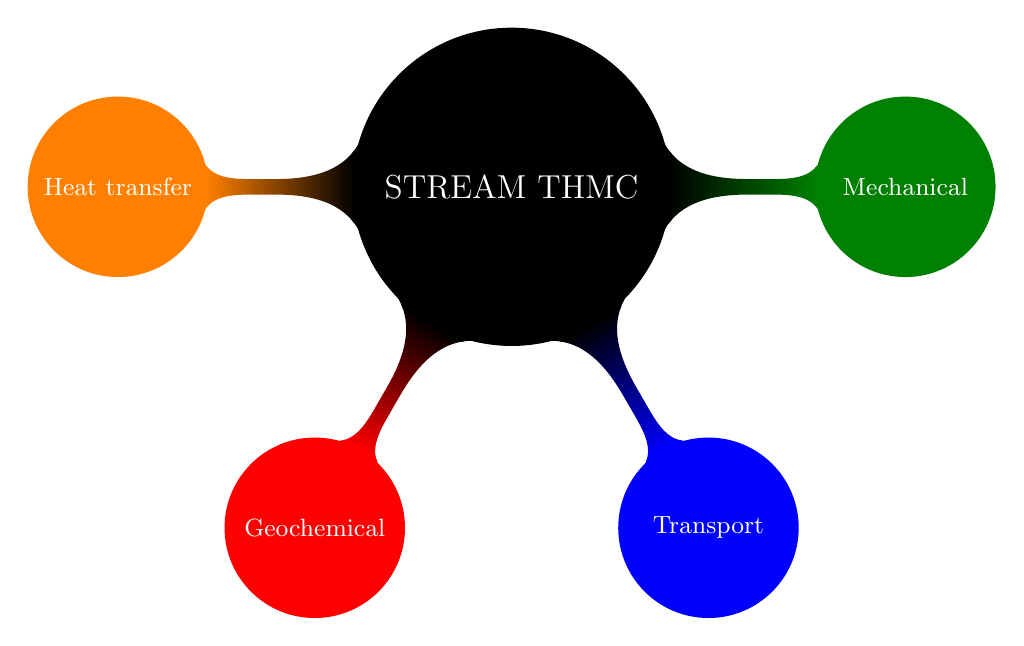
\begin{tikzpicture}
  \path[mindmap,concept color=black,text=white]
    node[concept] {STREAM THMC}
    [clockwise from=0]
    child[concept color=green!50!black] { node[concept] {Mechanical}    }  
    child[concept color=blue] {node[concept] {Transport}}
    child[concept color=red] { node[concept] {Geochemical} }
    child[concept color=orange] { node[concept] {Heat transfer} };
\end{tikzpicture}
\end{adjustbox}
\end{frame}
%%%%%%%%%%%%%%%%%%%%%%%%%%%%%%%%%%%%%%%%%%%%%%
\section{Mathematical model}
%%%%%%%%%%%%%%%%%%%%%%%%%%%%%%%%%%%%%%%%%%%%%%%
%%%%%%%%%%%%%%%%%%%%%%%%%%%%%%%%%%%%%%%%%
\begin{frame}{Poromechanics}
\begin{columns}
\begin{column}{0.4\textwidth}
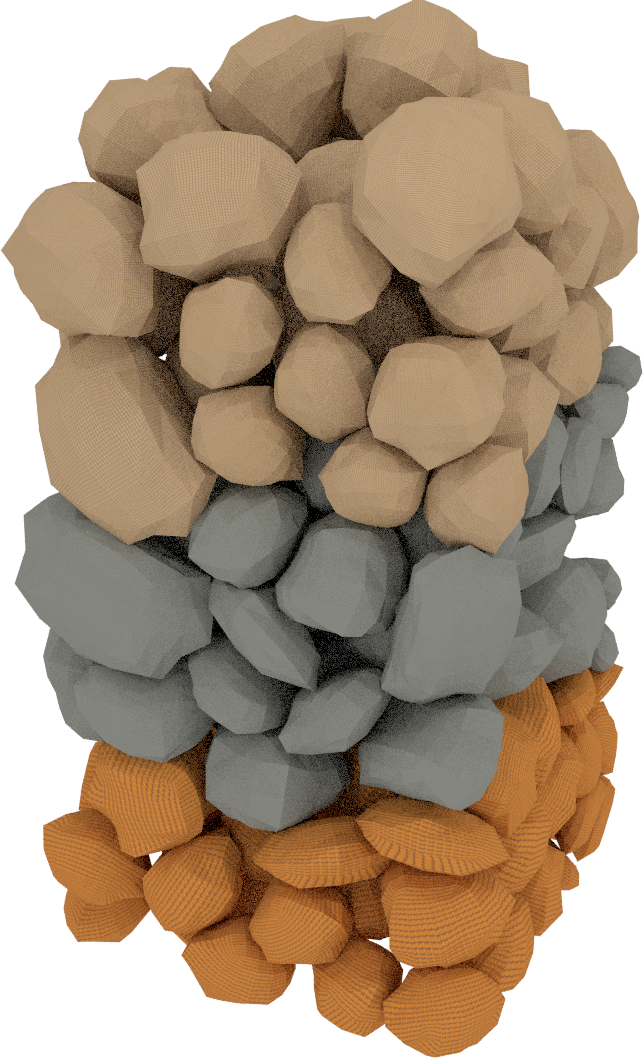
\includegraphics[width=0.9\columnwidth]{figure/poromech}
\end{column}
\begin{column}{0.4\textwidth}
	\begin{align*}
 	-\nabla \cdot \left(  2\mu\varepsilon (\mathbf{u}) + \nabla\cdot \mathbf{u}\right) + \alpha \nabla p=\rho\mathbf{g} \, ,\\
 	\partial_t \left(\frac{p}{M} + \alpha \nabla \cdot \mathbf{u}\right)+ \nabla\cdot \mathbf{u_d}=S_f\,,\\ 
 	\mathbf{K}^{-1}\mathbf{u_d} + \nabla p = \rho_f\mathbf{g}\,,
 \end{align*}
\end{column}
\end{columns}
\end{frame}
%%%%%%%%%%%%%%%%%%%%%%%%%%%%%%%%%%%%%%%%%%%%%%%%%
%%%%%%%%%%%%%%%%%%%%%%%%%%%%%%%%%%%%%%%%%
\begin{frame}{Temperature Dynamics}
\begin{columns}
\begin{column}{0.4\textwidth}
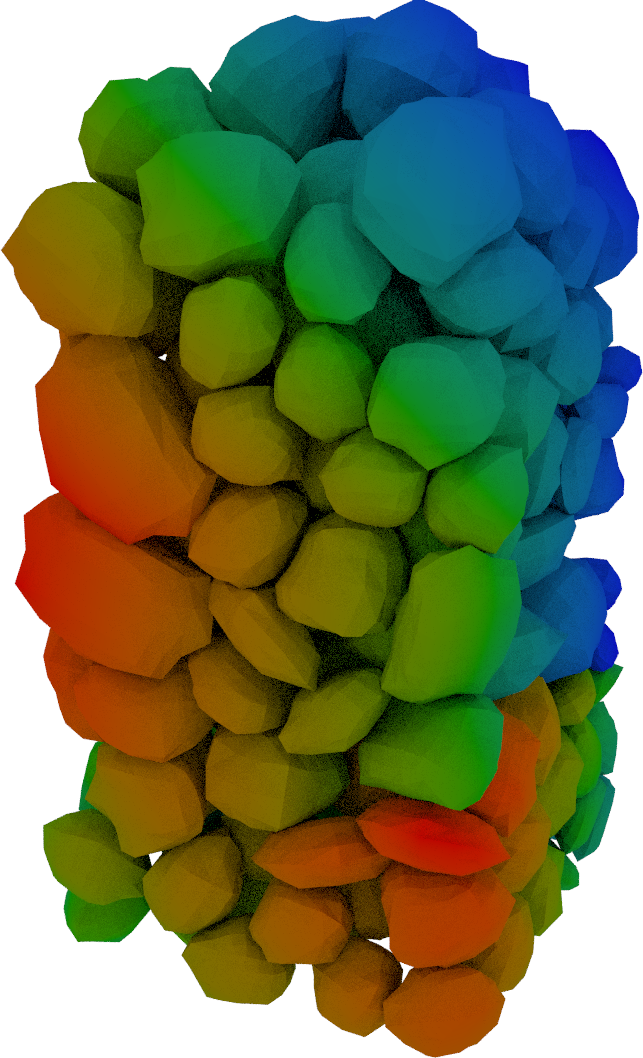
\includegraphics[width=0.9\columnwidth]{figure/poromechhot}
\end{column}
\begin{column}{0.4\textwidth}
	\begin{align*}
 	& C_T\frac{\partial T}{\partial t} - K_T \nabla^2 T \\ 
 	& +\left(  \phi\rho_l c_l \mathbf{v_l} 
 	+  (1 - \phi)\rho_s c_s \mathbf{v_s} \right)\cdot \nabla T
 	= Q\,.
 \end{align*}
\end{column}
\end{columns}
\end{frame}
%%%%%%%%%%%%%%%%%%%%%%%%%%%%%%%%%%%%%%%%%%%%%%%%%
%%%%%%%%%%%%%%%%%%%%%%%%%%%%%%%%%%%%%%%%%
\begin{frame}{Chemical transport}
\begin{columns}
\begin{column}{0.4\textwidth}
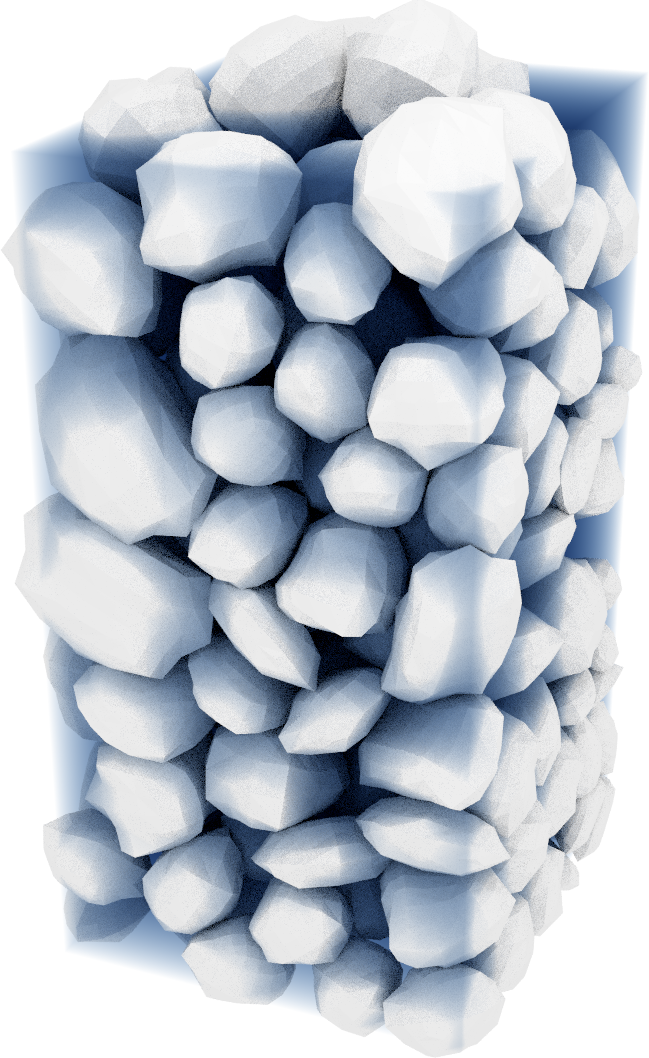
\includegraphics[width=0.9\columnwidth]{figure/poromechwater}
\end{column}
\begin{column}{0.4\textwidth}
	\begin{align*}
 	C_T\frac{\partial C}{\partial t} +
 	\mathbf{u_D} \cdot \nabla C- D\nabla^2 T 
 	= Q_c\,.
 \end{align*}
\end{column}
\end{columns}
\end{frame}
%%%%%%%%%%%%%%%%%%%%%%%%%%%%%%%%%%%%%%%%%%%%%%%%%
\begin{frame}{Ice fraction}
\setbeamercolor{block title}{bg=olive!50!white}
\setbeamercolor{block body}{bg=olive!30!white}
\begin{block}{Porosity}
\begin{equation*}
\theta_l =S_i \phi_i
\end{equation*} 
\end{block}
{
\setbeamercolor{block title}{bg=cerulean!50!white}
\setbeamercolor{block body}{bg=cerulean!30!white}
\begin{block}{Ice fraction}
%{\resizebox{1cm}{!}{
\begin{equation*}
\small
S_i=\left\{
\begin{aligned}
&1 \quad & T > T_L \,,\\
&(1-S_{lres})\exp\left[ - \left( \frac{T-T_L}{w}\right)^2 \right] +
S_{lres} \quad & T_L> T > T_{lres}\,,\\
&S_{lres}  \quad &  T < T_{lres}\,.
\end{aligned}
\right.
\end{equation*}
%}}
\end{block}
}
\end{frame}
%%%%%%%%%%%%%%%%%%%%%%%%%%%%%%%%%%%%%%%%%%%%%%%

\begin{frame}{Constitutive law}
\setbeamercolor{block title}{bg=cerulean!50!white}
\setbeamercolor{block body}{bg=cerulean!30!white}
\begin{block}{}
		\begin{equation*}
			\mu=1.002\, 10^{-3} \left( 1+ \alpha_1(T) +\alpha_2(C_M) \right)
		\end{equation*}
		 
		\begin{equation*}
			\rho_l =  \rho_0(1+\beta_1(T)+ \beta_2(C_M) )\, .
			\label{consrho}
		\end{equation*}%%%%%%%%%%%%%%%%%%%%%%%%%%%%%%%%%%%%%%%%
\end{block}
{
 \setbeamercolor{block title}{bg=olive!50!white}
\setbeamercolor{block body}{bg=olive!30!white}
\begin{block}{Permeability}
\begin{equation*}
k=k_pK; \, k_p=\left\{
\begin{aligned}
&1 \quad & T > T_L \,,\\
& \left( \frac{k_{min}-1}{T_l}\right)T +1 \quad & T_L> T > T_{lres}\,,\\
&k_{min}  \quad &  T < T_{lres}\,.
\end{aligned}
\right.
\end{equation*}
\end{block}
}
\end{frame}
%%%%%%%%%%%%%%%%%%%%%%%%%%%%%%%%%%%%%%%%%%%%%%%
%%%%%%%%%%%%%%%%%%%%%%%%%%%%%%%%%%%%%%%%%
\begin{frame}{Coupled model}
Poromechanics - Temperature Dynamics - Chemical transport
	\begin{equation*}
	 \begin{split}
	   	-\nabla \cdot \left(  2\mu\varepsilon (\mathbf{u}) + \lambda\nabla\cdot \mathbf{u}\right) + \alpha \nabla p=\rho\mathbf{g} \label{momentum}\, ,\\
 	\partial_t \left(\frac{p}{M} + \alpha \nabla \cdot \mathbf{u}\right)+ \nabla\cdot \mathbf{u_d}=S_f\,,\\ 
 	\mathbf{K}^{-1}\mathbf{u_d} + \nabla p = \rho_f\mathbf{g}\,.\\
	 \end{split}
	\end{equation*}
	\begin{equation*}
 	C_D\frac{\partial C}{\partial t} +
 	\mathbf{u_D} \cdot \nabla C- D\nabla^2 C 
 	= Q_c\,.
 	\end{equation*}
	\begin{equation*}
 	C_T\frac{\partial T}{\partial t} +
 	\left(  \phi\rho_l c_l \mathbf{v_l} 
 	+  (1 - \phi)\rho_s c_s \mathbf{v_s} \right)\cdot \nabla T- K_T \nabla^2 T 
 	= Q\,.
 	\end{equation*}
\end{frame}
%%%%%%%%%%%%%%%%%%%%%%%%%%%%%%%%%%%%%%%%%%%%%%%%%
%%%%%%%%%%%%%%%%%%%%%%%%%%%%%%%%%%%%%%%%%
\begin{frame}{Coupled model}
Poromechanics - Temperature Dynamics - Chemical transport
	\begin{equation*}\boxed{
	 \begin{split}
	   	-\nabla \cdot \left(  2\mu\varepsilon (\mathbf{u}) + \lambda\nabla\cdot \mathbf{u}\right) + \alpha \nabla p=\rho\mathbf{g} \label{momentum}\, ,\\
 	\partial_t \left(\frac{p}{M} + \alpha \nabla \cdot \mathbf{u}\right)+ \nabla\cdot \mathbf{u_d}=S_f\,,\\ 
 	\mathbf{K}^{-1}\mathbf{u_d} + \nabla p = \rho_f\mathbf{g}\,.\\
	 \end{split}}{orange}
	\end{equation*}
	\begin{equation*}\boxed{
 	C_D\frac{\partial C}{\partial t} +
 	\mathbf{u_D} \cdot \nabla C- D\nabla^2 C 
 	= Q_c\,.}{blue}
 	\end{equation*}
	\begin{equation*}\boxed{
 	C_T\frac{\partial T}{\partial t} +
 	\left(  \phi\rho_l c_l \mathbf{v_l} 
 	+  (1 - \phi)\rho_s c_s \mathbf{v_s} \right)\cdot \nabla T- K_T \nabla^2 T 
 	= Q\,.}{green}
 	\end{equation*}
\end{frame}
%%%%%%%%%%%%%%%%%%%%%%%%%%%%%%%%%%%%%%%%%%%%%%%%%
\section{1D prototype}
% %%%%%%%%%%%%%%%%%%%%%%%%%%%%%%%%%%%%%%%%%%%%%%%%%%%%%%%%%%%%5
\begin{frame}{STREAM 1D THMC (Matlab prototype) Frozen Geco}
\ 
\\  
\begin{columns}
\begin{column}{0.6\textwidth}
Momentum
\begin{equation*}
\phi(u^l-u^s)=-\frac{K}{\mu^l}\left(\frac{d p^l}{dz}  -\rho^l \mathbf{g}\right)
\end{equation*}
Geomechanics
\begin{equation*}
\frac{d\phi_M}{dt}=-\beta(\phi_0-\phi_f)\exp(-\beta\sigma)\frac{d\sigma}{dt}
\end{equation*}
Heat transfer
\begin{equation*}
C_t\frac{dT}{dt} + \rho c \mathbf{u}_d\cdot \frac{dT}{dz}  - K \frac{d T^2}{dz^2} =0
\end{equation*}
Chemical Transport
\begin{equation*}
\phi \rho_l \frac{\partial C}{\partial t} +  \rho_l \mathbf{u}_d\cdot
\frac{dC}{dz}  = \phi \rho_l D \frac{d C^2}{dz^2}
\end{equation*}
% \begin{equation*}
% (\phi_m - \phi_f)\exp \left(-\frac{z_t-z}{\phi_c}\right) + \phi_f
% \end{equation*}
\end{column}
\begin{column}{0.5 \textwidth}
$u^l$ liquid velocity\\
$u^s$ solid velocity\\
$u_d$ Darcy velocity\\
$\sigma$ axial effective stress\\
\vspace{1cm}
 \begin{itemize}
  \item Mono dimensional domain
  \item Transient simulation
  \item Ice formation
  \item Complex constitutive models
 \end{itemize}
\end{column}
\end{columns}
\end{frame}
%%%%%%%%%%%%%%%%%%%%%%%%%%%%%%%%%%%%%%%%%%%%%%%%%%%%%%%%%%%%%%%%
\begin{frame}{geco}
\begin{columns}
\begin{column}{0.2\textwidth}
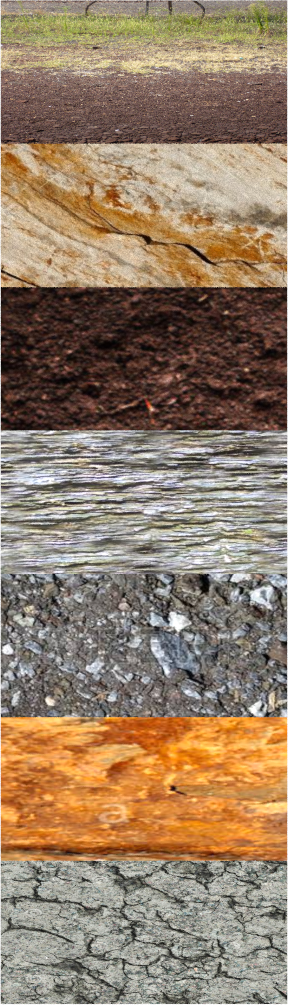
\includegraphics[width=0.9\columnwidth]{figure/gecoover}
\end{column}
\begin{column}{0.7\textwidth}
\begin{tabular}{lccc}
Materials &  (Pa$^{-1}$) & K ($m^2$) & h (m)\\ 
7 Aquifer & $10^{-9}$ & $10^{-12} $ & $825$\\
6 Shale & $ 5 \, 10^{-8}$ & $ 10^{-16} $  $400$\\
5 Aquifer & $10^{-9}$ & $10^{-13} $ & $825$\\
4 Shale & $ 10^{-8}$ & $ 10^{-17} $ & $500$\\
3 Aquifer & $5 \, 10^{-10}$ & $10^{-14} $ & $825$\\
2 Shale & $5 \, 10^{-9}$ & $10^{-18} $ & $800$\\
1 Aquifer & $5 \, 10^{-10}$ & $10^{-14} $ & $825$\\
\end{tabular}
\end{column}
\end{columns}
\end{frame}
%%%%%%%%%%%%%%%%%%%%%%%%%%%%%%%%%%%%%
%%%%%%%%%%%%%%%%%%%%%%%%%%%%%%%%%%%%%%%%%%
\begin{frame}{Set up}
\begin{columns}
\uncover<2->{
\begin{column}{0.25\textwidth}
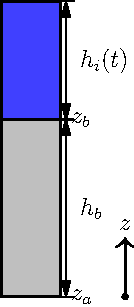
\includegraphics[width=0.8\columnwidth]{figure/test_case}
\end{column}
}
\uncover<3->{
\begin{column}{0.7\textwidth}
\ \\
\vspace{0.2cm}
\begin{align*}
& h_b(t=0)=5000m\\
& D  =10^{-10} m^2/s \\
& C (t=0) = -\frac{(0.4-0.1)}{h_b}z + 0.1\\ 
& C (z_a, t) =0, \partial C / \partial z | _{z_b} =0\\
& dt = 0.3 y , \quad \Delta t =10 y\\
& h_s=500 m , 2000 m , \frac{2000}{\Delta t}t 
\end{align*}
\end{column}
}
\end{columns}
\tiny{
\begin{thebibliography}{99} % Beamer does not support BibTeX so references must be inserted manually as below
\bibitem[Smith, 2012]{p1} Bense, V. F., and M. A. Person. (2008)
\newblock Transient hydrodynamics within intercratonic sedimentary basins during glacial cycles.
\newblock \emph{Journal of Geophysical Research} 113.F4 .
\end{thebibliography}
}
\end{frame}
%%%%%%%%%%%%%%%%%%%%%%%%%%%
\begin{frame}
\frametitle{Test case}\uncover<2->{
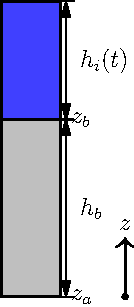
\includegraphics[width=0.2\textwidth]{figure/test_case}\uncover<3->{
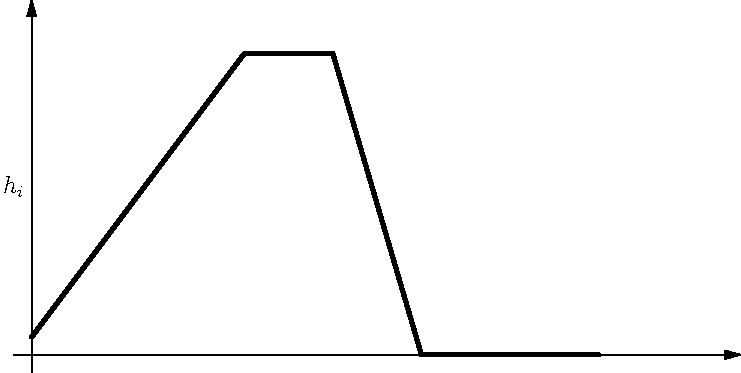
\includegraphics[width=0.7\textwidth]{figure/hice}\\}}
{\centering
$\Delta t_{tot} = 32 Ky \qquad \Delta t _0 =0.1y \qquad \Delta t_{max}= 0.1Ky$\\
$ h_b(t=0)=5000m \qquad D  =10^{-10} m^2/s  \qquad \theta_{l}=S_l\phi$
}
\begin{thebibliography}{99} 
\bibitem[Smith, 2012]{p1} Bense, V. F., and M. A. Person. (2008)
\newblock Transient hydrodynamics within intercratonic sedimentary basins during glacial cycles.
\newblock \emph{Journal of Geophysical Research} 113.F4 .
\bibitem[jenkins2011convection]{beh}Jenkins, A
\newblock Convection-driven melting near the grounding lines of ice shelves and
  tidewater glaciers.
\newblock {\em Journal of Physical Oceanography}, 41(12):2279--2294, 2011.
\end{thebibliography}
\end{frame}
%%%%%%%%%%%%%%%%%%%%%%%%%%%
\begin{frame}
\frametitle{Test case}\uncover<1->{
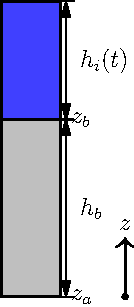
\includegraphics[width=0.2\textwidth]{figure/test_case}\uncover<1->{
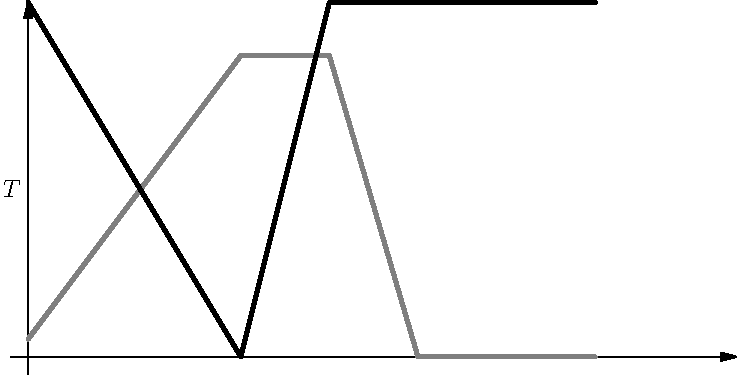
\includegraphics[width=0.7\textwidth]{figure/tempice}\\}}
{\centering
$\Delta t_{tot} = 32 Ky \qquad \Delta t _0 =0.1y \qquad \Delta t_{max}= 0.1Ky$\\
$ h_b(t=0)=5000m \qquad D  =10^{-10} m^2/s  \qquad \theta_{l}=S_l\phi$
}
\begin{thebibliography}{99} 
\bibitem[Smith, 2012]{p1} Bense, V. F., and M. A. Person. (2008)
\newblock Transient hydrodynamics within intercratonic sedimentary basins during glacial cycles.
\newblock \emph{Journal of Geophysical Research} 113.F4 .
\bibitem[jenkins2011convection]{beh}Jenkins, A
\newblock Convection-driven melting near the grounding lines of ice shelves and
  tidewater glaciers.
\newblock {\em Journal of Physical Oceanography}, 41(12):2279--2294, 2011.
\end{thebibliography}
\end{frame}
%%%%%%%%%%%%%%%%%%%%%%%%%%%
\begin{frame}{Test cases}
\begin{tabular}{c|c|c}
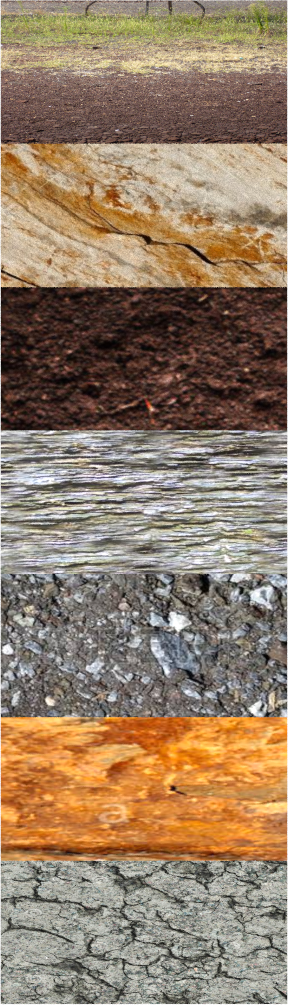
\includegraphics[width=0.19\textwidth]{figure/gecoover}&
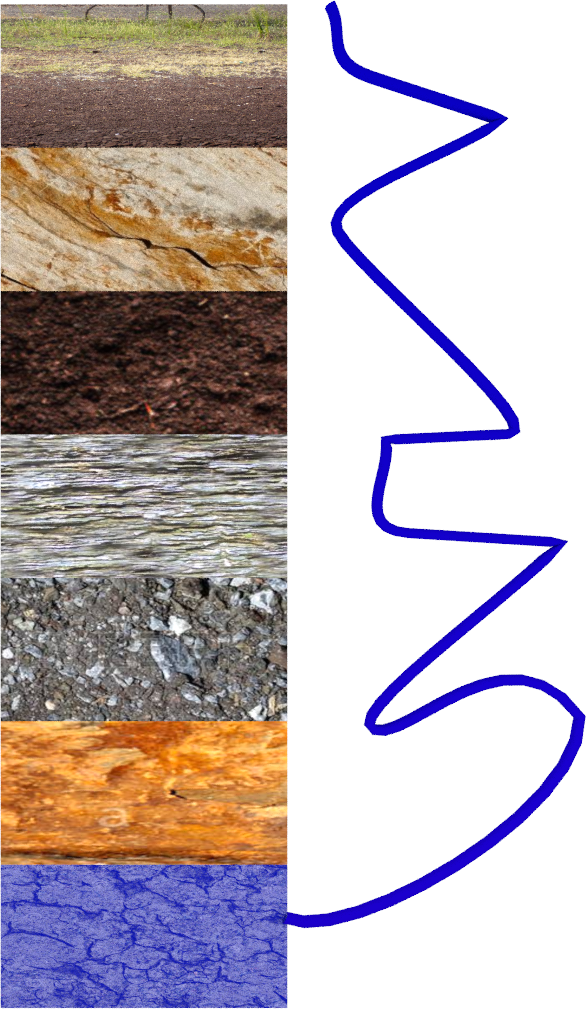
\includegraphics[width=0.386\textwidth]{figure/coldchannel}&
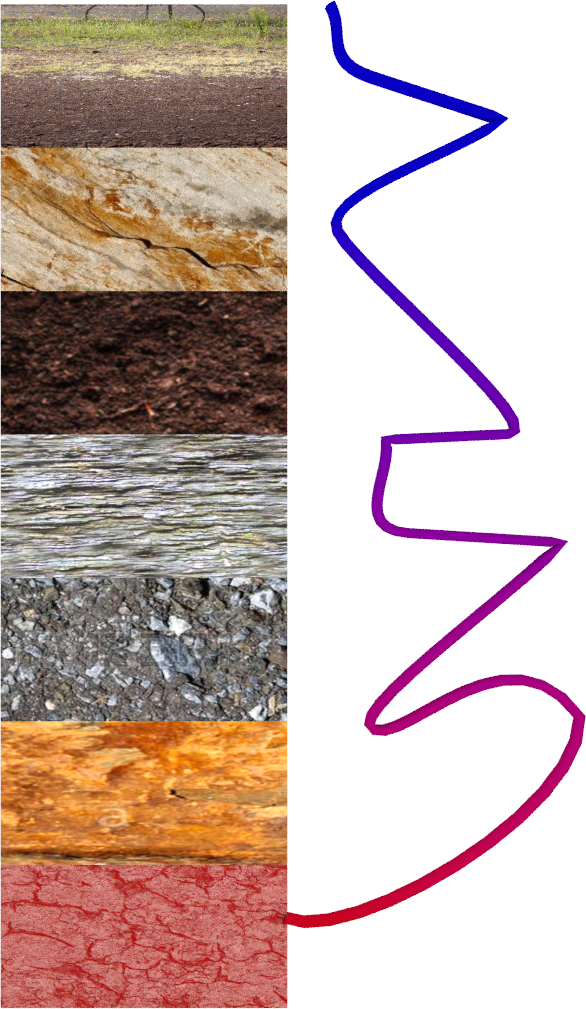
\includegraphics[width=0.386\textwidth]{figure/hotchannel}\\
A & B & C 
\end{tabular}
\end{frame}




%%%%%%%%%%%%%%%%%%%%%%%%%%%%%%%%%%%%%%%
\section{Numerical Plattofrm}
%%%%%%%%%%%%%%%%%%%%%%%%%%%%%%%%%%%%%%%%%%%%%%%
%%%%%%%%%%%%%%%%%%%%%%%%%%%%%%%%%%%%
\begin{frame}{Numerical platform}
\begin{columns}
\begin{column}{0.45\textwidth}

\includegraphics[width=0.8\columnwidth]{figure/logogetfem}
\begin{block}{GetFem}
\begin{itemize}
\item c++ finite element platform
\item Generic assembly language
\item Level-set and finite element cut 
	by one or several level-set (Xfem) 
\end{itemize}
\end{block}
\end{column}
\begin{column}{0.45\textwidth}
\begin{block}{SAMG library}
Algebraic Multigrid Methods for Systems
\begin{itemize}
\item solution of large linear systems
\item higly scalable
\item easy to integrate
\end{itemize}
\end{block}
\end{column}
\end{columns}
\end{frame}
%%%%%%%%%%%%%%%%%%%%%%%%%%%%%%%%%%%%%%%%%%%%%
%%%%%%%%%%%%%%%%%%%%%%%%%%%%%%%%%%%%%
\begin{frame}{Geometric VS Algebraic}
\centering
\vfill
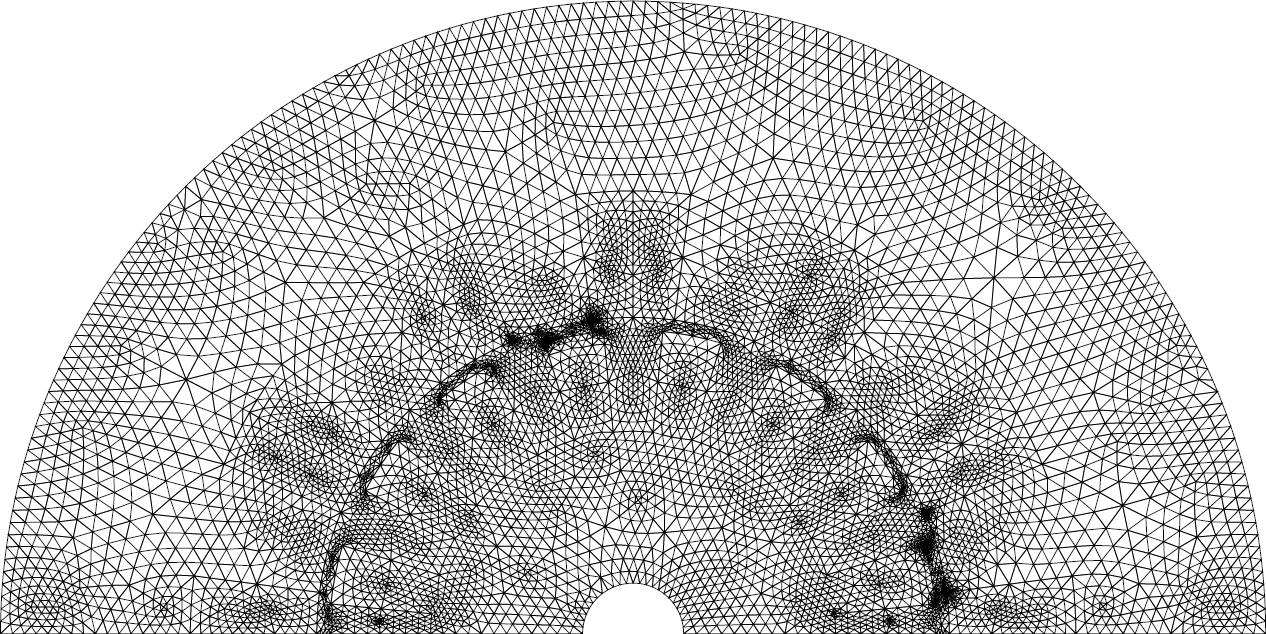
\includegraphics[width=0.7\textwidth]{figure/compex1.png}
\vfill
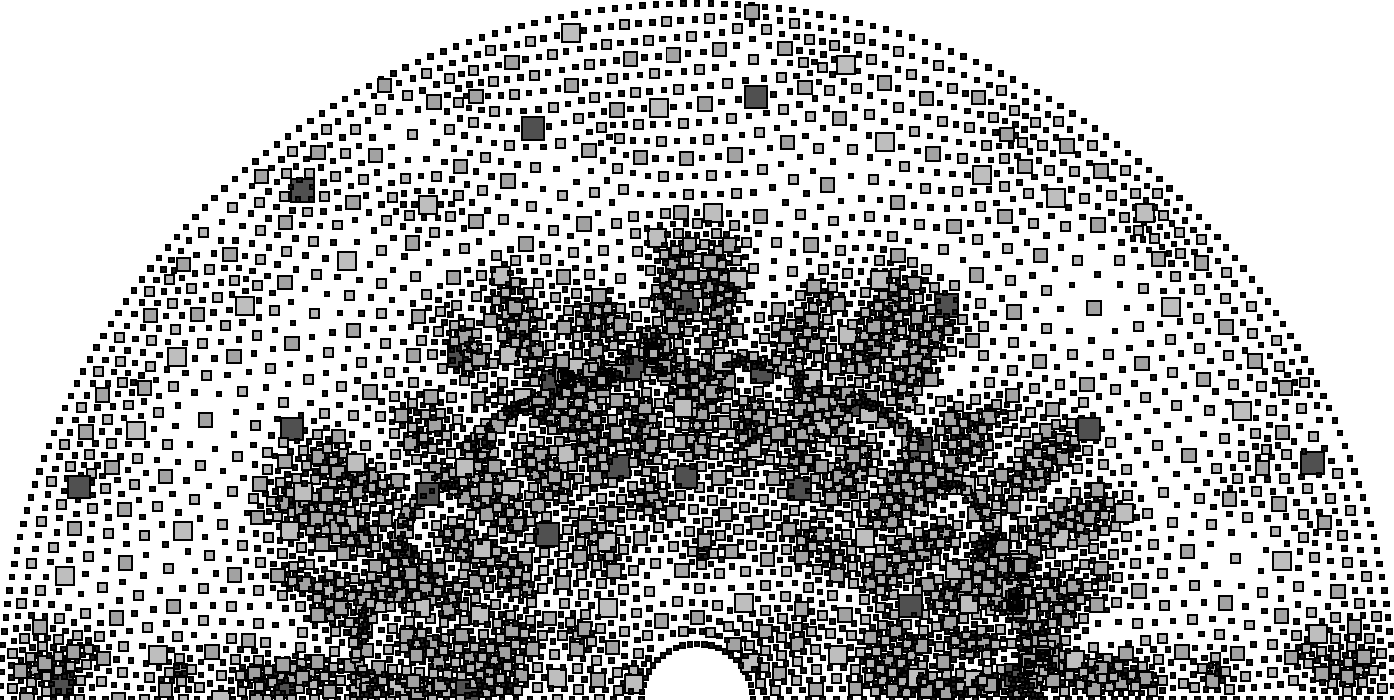
\includegraphics[width=0.7\textwidth]{figure/compex2.png}
\vfill
\end{frame}
%%%%%%%%%%%%%%%%%%%%%%%%%%%%%%%%%%%%%%
%%%%%%%%%%%%%%%%%%%%%%%%%%%%%%%%%%%%%%%%%%%%%
\begin{frame}{Integration}
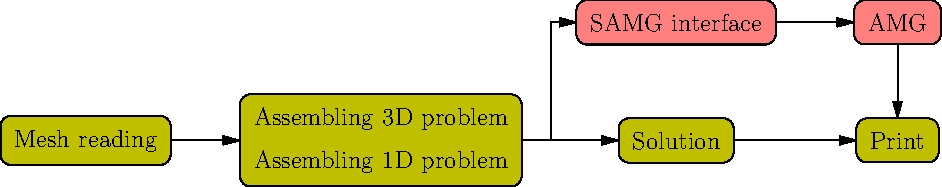
\includegraphics[width=0.9\textwidth]{figure/flowchart}
\begin{itemize}
\item Simple interface (CSR matrix)
\item Same programming language
\end{itemize}
\end{frame}
%%%%%%%%%%%%%%%%%%%%%%%%%%%%%%%%%%%%%%%%%%%%%%%%%%%%%%
\begin{frame}{Benchmark}
 \begin{columns}
  \begin{column}{0.45\textwidth}
    \begin{align*}
 	-\nabla \cdot \left(  2\mu\varepsilon (\mathbf{u}) + \nabla\cdot \mathbf{u}\right) + \alpha \nabla p=\mathbf{0} \, ,\\
 	\partial_t \left(\frac{p}{M} + \alpha \nabla \cdot \mathbf{u}\right)+ \nabla\cdot \mathbf{u_d}=S_f\,,\\ 
 	\mathbf{K}^{-1}\mathbf{u_d} + \nabla p = \mathbf{0}\,,\\
 \end{align*}
  \end{column}
    \begin{column}{0.45\textwidth} 
    \\ 
  {\bf Mandel benchmark}
    \centering
    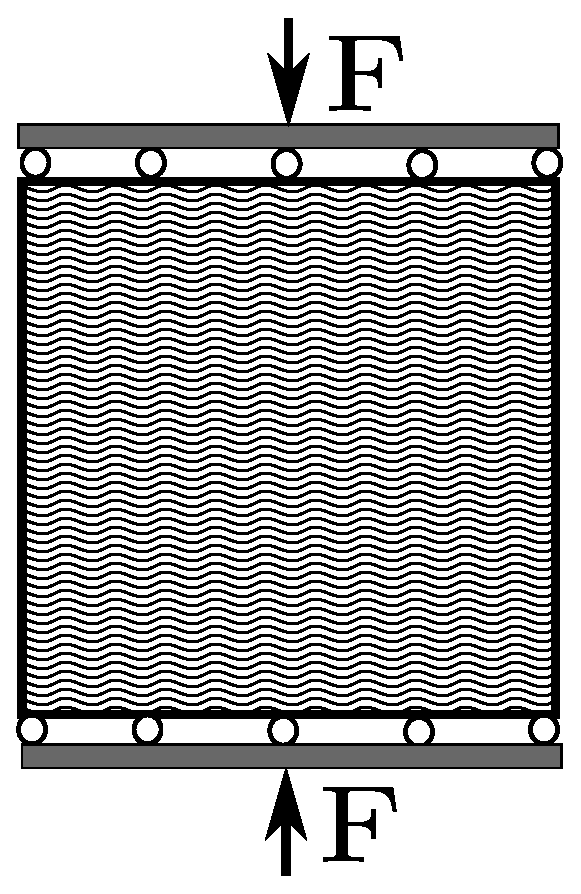
\includegraphics[width=0.7\columnwidth]{figure/madleysvg}
    \end{column}
 \end{columns}

 \begin{itemize}
 \item 
 Both, Jakub Wiktor, et al. 
 \textit{Robust fixed stress splitting for Biot's equations in heterogeneous media.
 Applied Mathematics Letters 2017.}
  \item
Cui, L., et al.
  \textit{Finite element analyses of anisotropic 
  poroelasticity: a generalized Mandel's 
  problem and an inclined borehole problem.,
  International Journal for Numerical and Analytical Methods in Geomechanics,
  1996.} 
  \end{itemize}

\end{frame}



%%%%%%%%%%%%%%%%%%%%%%%%%%%%%%%%%%%%%%%%%%%%%%%
\section{Conclusion}
%%%%%%%%%%%%%%%%%%%%%%%%%%%%%%%%%%%%%%%%%%%%%%%








\end{document}
